\subsubsection{Gradientenindex}

Das Gradientenindexprofil bittet mit bis zu 10 Gigabit/s auf 100m deutlich
höhere Bitraten als das Stufenindexprofil. Beim Gradientenindex nimmt der
Brechungsindex vom Mantel bis zur Mitte des Kern kontinuierlich zu (siehe
\autoref{fig:pofgi} Spalte Brechungsindex). \autoref{fig:pofgi} zeigt ebenfalls
in der Spalte Längsschnitt den daraus resultierenden Lichtstrahlenverlauf.
Dieser verläuft, im Gegensatz zu der geraden Lichtausbreitung beim Stufenindex,
sinusförmig. Dadurch werden geringere Laufzeitunterschiede ermöglicht und die
Frequenz der Lichtimpulse kann erhöht werden. Außerdem wird bei der
Gradientenfaser eine Dämpfung von unter 20 dB/km erreicht (siehe
\autoref{fig:pofgidaempfung}. Dies ist ein ehrheblicher Sprung über der
Dämpfung einer Stufenfaser mit ca 100 dB/km (siehe \autoref{fig:pofdaempfung}).
Aus den beiden Gründen ist die Bandbreite einer Faser mit Gradientenindex
significant höher als die einer einer Faser mit Stufenindex. Aufgrund der hohen
Bitraten werden Gradientenfasern im \shorthandoff{"}"Local Area
Network"\shorthandon{"} (LAN) eingesetzt. Als Kernmaterial wird hier der
Kunststoff CYTOP\textsuperscript{\textregistered} der Asahi Glass Company
verwendet (siehe \autoref{subsec:pofcytop}). \cite{pofacgif}

\begin{figure}[h]
    \begin{center}
        \begin{minipage}[t]{0.4\textwidth}
            \begin{center}
                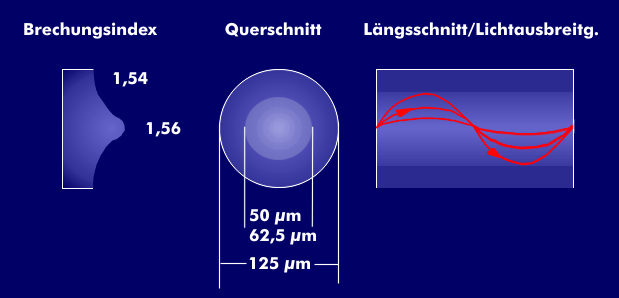
\includegraphics[height=0.1\textheight]{Bilder/Optische_Wellenleiter_Die_Polymer_Optische_Faser/Brechzahlprofile/pofgi.png}
                \caption[Aufbau des Gradientenindexprofils \newline \url{ITWissen}]{Aufbau des Gradientenindexprofils}
                \label{fig:pofgi}
            \end{center}
        \end{minipage}
        \hspace{0.025\textwidth}
        \begin{minipage}[t]{0.4\textwidth}
            \begin{center}
                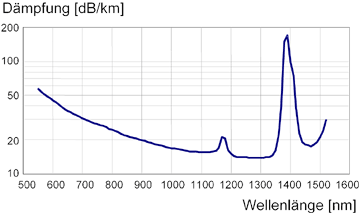
\includegraphics[height=0.1\textheight]{Bilder/Optische_Wellenleiter_Die_Polymer_Optische_Faser/Brechzahlprofile/pofgidaempfung.png}
                \caption[Dämpfung bei einer Gradientenfaser \newline \url{POFAC}]{Dämpfung bei einer Gradientenfaser}
                \label{fig:pofgidaempfung}
            \end{center}
        \end{minipage}
    \end{center}
\end{figure}

%TODO: Get url
